% Asset ID: AS2ConstantAccelerationTikZ-001
% File: tikz/AS2ConstantAccelerationTikZ-001.tex
% Source: MechYr1 Chapter 9 Constant Acceleration PDF and teacher transcript
% Related lesson section: Core Theory - SUVAT Derivations
% Purpose: Clean velocity-time graph used to derive v = u + at and s = ((u+v)/2)t.
% Related LO IDs: AS2-KIN-LO002, AS2-KIN-LO003
% Status: Written

\documentclass[tikz,border=10pt]{standalone}
\usepackage{amsmath}
\usepackage{tikz}
\usetikzlibrary{arrows.meta,calc,patterns}

\begin{document}
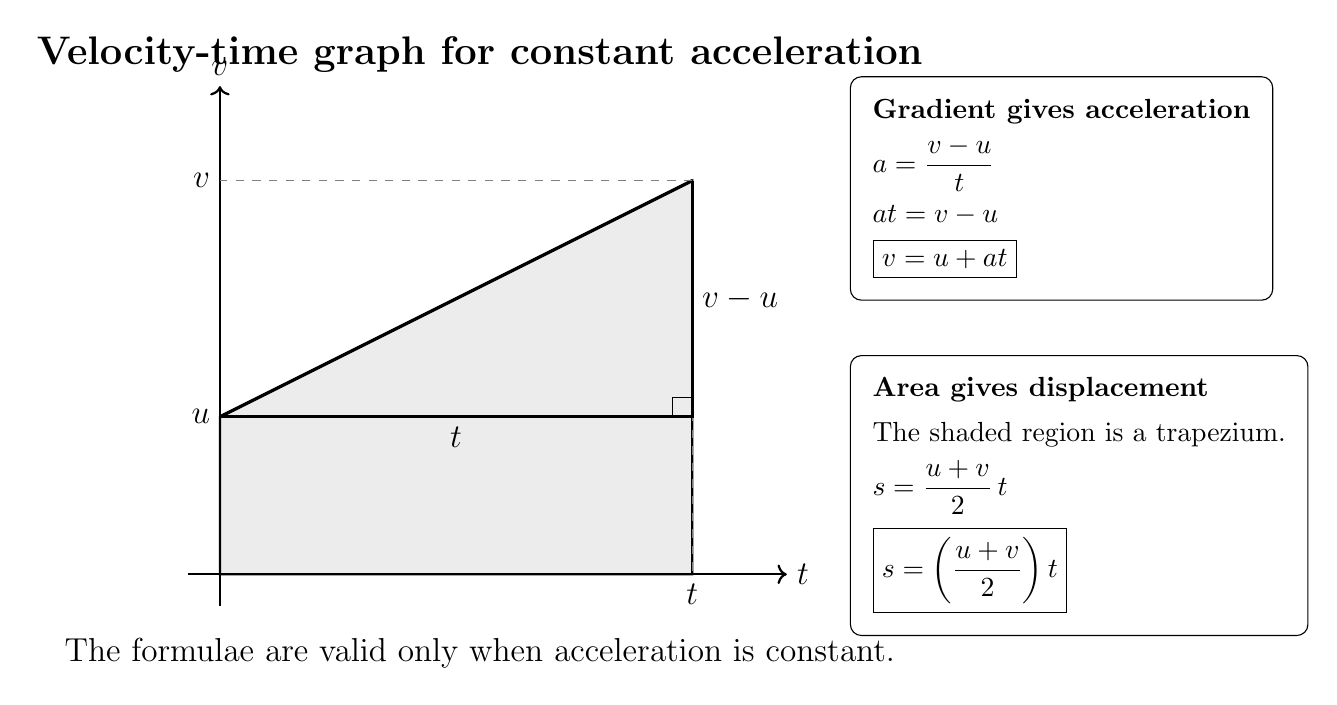
\begin{tikzpicture}[
    axis/.style={->, thick},
    guide/.style={dashed, gray},
    graphline/.style={very thick},
    labeltext/.style={font=\large},
    formulabox/.style={draw, rounded corners, align=left, inner sep=8pt}
]
\coordinate (O) at (0,0);
\coordinate (A) at (0,2);
\coordinate (B) at (6,5);
\coordinate (C) at (6,0);
\draw[axis] (-0.4,0) -- (7.2,0) node[right, labeltext] {$t$};
\draw[axis] (0,-0.4) -- (0,6.2) node[above, labeltext] {$v$};
\fill[gray!15] (O) -- (A) -- (B) -- (C) -- cycle;
\draw[thick] (O) -- (A) -- (B) -- (C) -- cycle;
\draw[graphline] (A) -- (B);
\draw[guide] (B) -- (C);
\draw[guide] (B) -- (0,5);
\node[left, labeltext] at (A) {$u$};
\node[left, labeltext] at (0,5) {$v$};
\node[below, labeltext] at (C) {$t$};
\coordinate (D) at (6,2);
\draw[very thick] (A) -- (D) -- (B);
\node[below, labeltext] at ($(A)!0.5!(D)$) {$t$};
\node[right, labeltext] at ($(D)!0.5!(B)$) {$v-u$};
\draw ($(D)+(-0.25,0)$) -- ($(D)+(-0.25,0.25)$) -- ($(D)+(0,0.25)$);
\node[formulabox, anchor=west] at (8.0,4.9) {\textbf{Gradient gives acceleration}\\[4pt]
$\displaystyle a=\frac{v-u}{t}$\\[4pt]
$\displaystyle at=v-u$\\[4pt]
$\displaystyle \boxed{v=u+at}$};
\node[formulabox, anchor=west] at (8.0,1.0) {\textbf{Area gives displacement}\\[4pt]
The shaded region is a trapezium.\\[4pt]
$\displaystyle s=\frac{u+v}{2}\,t$\\[4pt]
$\displaystyle \boxed{s=\left(\frac{u+v}{2}\right)t}$};
\node[align=center, font=\Large\bfseries] at (3.3,6.6) {Velocity-time graph for constant acceleration};
\node[align=center, font=\large] at (3.3,-1.0) {The formulae are valid only when acceleration is constant.};
\end{tikzpicture}
\end{document}
